\newpage
\section{Generierung der Simulationsumgebung}
\label{generierung_sim}
Die Generierung der Trainingsumgebung ist ein Hauptaspekt des Projekts. Der Agent soll in einer möglichst realistischen Supermarkt-Simulation lernen einen Einkauf abzuschließen. Hierfür werden Regeln und Annahmen benötigt auf deren Basis die Generierung erfolgt. 
\\
Um die Annahmen besser nachvollziehen zu können, muss kurz erklärt werden, wie die Erstellung der Umgebung ablaufen soll. Grundsätzlich wird das Umfeld mithilfe mehrerer 2D Grids (dt.: Gitternetze) generiert. Diese beinhalten Informationen über die Position der Regale und Hindernisse. Mit diesen Daten werden dann Assets wie modellierte Regale geladen, welche an die gespeicherte Position gesetzt werden. Somit wird eine dreidimensionale Umgebung erstellt. Die Regale sind dabei modulare Elemente. Ziel ist es in jeder Iteration der Erstellung des Supermarkts eine neue zufällige Umgebung zu generieren, so dass der Agent keine Umgebung einfach auswendig lernt. Diese Zufälligkeit ist jedoch nur begrenzt umsetzbar und es kann nicht gewährleistet werden, dass die Umgebung nicht schon einmal so erstellt wurde. Dies stellt kein Problem dar, solange sich das Umfeld zwischen jeder Iteration ausreichend verändert. 
Im Folgenden werden die verwendeten Annahmen, sowie die Visualisierung der Umgebung erklärt. Zusätzlich wird genauer beschrieben, wie das Simulationsumfeld generiert und genutzt wird.

\subsection{Getroffene Annahmen für die Implementierung des Projekts}
\label{annahmen}
Für die Implementierungen dieses Projekts wurden diverse Annahmen getroffen, um die Modellierung dieser Aufgabe zu vereinfachen und überhaupt erst zu ermöglichen. Die Annahmen können hierbei in zwei Bereiche unterteilt werden. Zum einen betreffen diese die Strukturierung des Supermarktes. Zum anderen die Aktionen und die Sensorik des Agenten.
\\
Um die Simulation des Supermarktes in der Wirklichkeit zu verankern, habe ich mir mehrere Supermärkte angeschaut und den hier ansässigen Edeka ausgemessen. Dabei habe ich einige grundsätzliche Informationen zusammentragen können. 
\\
\begin{itemize}
	\item Die Abstände zwischen den Regalen liegen bei ungefähr 1.8 Metern, hierbei gibt es einige wenige Ausnahmen in Verbindung mit Aktionsaufstellern, diese werden aber außenvorgelassen.
	\item Strukturell beginnen die meisten Supermärkte mit frischen Produkten wie Obst, Gemüse, Brot, usw. Danach folgen häufig Kühlbereiche mit Fertigprodukten. Daraufhin länger haltbare Nahrungsmittel wie Süßigkeiten, Dosen, orientalische Produkte, usw. Zum Schluss folgen oft Getränke.
	\item Es gibt keine Sackgassen. Der Weg in das Abteil ist nie der einzige weg hinaus.
	\item Meist wird versucht ein möglichst hohes Maß an Abdeckung mit Regalen zu erreichen.
\end{itemize}
\noindent
\\
Auch wenn dies im Realen nicht immer gilt, wird für die Simulation angenommen, dass der Grundschnitt des Supermarktes sowie die Aufteilungen der Abteile quadratisch oder rechteckig sind. Die Grundfläche wird aus dem zweiten Stichpunkt abgeleitet, in vier Abteile aufgeteilt. Dazu gehören Eingang, Obst und Gemüse Bereich, Abteil mit länger haltbare Güter und Getränke Bereich. 
\\
Des Weiteren wurde für die Berechnung der Wegplanung angenommen, dass der Supermarkt mit der derzeitigen Regalstruktur kartografiert wurde. Zu dieser Karte gehören nur statische Elemente, die sich über die Zeit hinweg nicht ändern. Hindernisse wie Einkaufswägen und Pappboxen mit neuen Artikeln werden nicht miteinbezogen. Sollte sich die Regalanordnung ändern, muss auch die Karte erneuert werden. Ein Ansatz mit einer dynamischen Karte, in der Hindernisse während des Trainingsprozesses vom Agenten hinzugefügt oder gelöscht werden, wird in dieser Arbeit nicht betrachtet. Grundlage hierfür ist, einerseits die Rechenersparnis hinsichtlich der festgelegten Wegplanung. Andererseits ist die Betrachtung der Reaktion des Agenten auf unbekannte Hindernisse ein wichtiger Bestandteil der Arbeit. Das Kartografieren des Supermarktes ist simpel und realistisch umsetzbar. Jedoch gilt dies nicht für die Position der Artikel innerhalb des Supermarktes. Hierfür wird angenommen, dass eine Datenbank besteht, die diese Position eingespeichert hat und innerhalb der Karte darstellen kann. Diese Annahme ist eher unrealistisch, da die Datenbank ständig angepasst werden müsste, sobald die Produkte innerhalb der Regale umsortiert werden, oder neue Artikel hinzukommen. Des Weiteren ist dies besonders fehleranfällig, da der Agent davon ausgeht, dass der ihm übergebene Weg, der Richtige ist. Falls aber die Datenbank nach dem Umräumen nicht vollständig angepasst wurde, würde der Agent ein falsches Produkt einsammeln. Dennoch wurde diese Annahme getroffen, um in der vorgegebenen Zeit dieses Projekt umsetzen zu können. Eine Alternative zu diesem Ansatz, wäre die Entwicklung einer Künstlichen Intelligenz, welche die Produkte mithilfe einer Kamera erkennen kann. Ohne die potenziellen Probleme dieser Vorgehensweise zu beschreiben, wäre hierfür zunächst ein Datensatz mit tausenden Bildern der jeweiligen Produkte aus verschiedenen Perspektiven notwendig. Die Implementierung einer solchen KI als Instanz vor der eigentlichen Untersuchung übersteigt den Rahmen einer Masterarbeit. 
\\
Zusätzlich wird das Einsammeln der Artikel simplifiziert und dabei wird getestet, ob der Roboter zur berechneten Position fährt. Das physische Einsammeln von Objekten verschiedener Größe, während der Roboter nicht unbedingt perfekt ausgerichtet ist, ist hochkomplex, weswegen diese Form der Vereinfachung gewählt wurde.
\\
Des Weiteren gibt es zusätzliche Anpassungen, um die Berechnung der Simulation zu optimieren. Für die Kollisionsberechnung der Regale und der Kasse wurde jeweils eine große Hitbox benutzt. Für mehr Realismus hätte man hier die genau Form der Regale durch Hitboxen nachbauen können. 
\\
Zusätzlich wurden keine zufälligen Fehler zu den Sensordaten und auch der Steuerung hinzugefügt. Alle Berechnungen wurden genau übergeben. Grund hierfür war, dass der Agent lange kein sinnvolles Verhalten trainiert hat und das Hinzufügen von Fehlern keinen Mehrwert gebracht hätte.
\\
Bei der Sensorik wurden zusätzlich noch weitere Vereinfachungen gewählt. Für das Projekt wurden keine realistisch funktionierenden Lidar- oder Ultraschallwellensensoren benutzt. Stattdessen wurde die Ray Perception Sensor Komponente verwendet, welche ML-Agents mitliefert. Diese ist für die Nutzung mit Agents ausgelegt und arbeitet ähnlich wie ein Lidar. Darum liegt der Grad der Abstraktion für diese Arbeit im Rahmen. Zusätzlich wird angenommen, dass die Position des Agenten sowie die Position des Ziels genau bekannt ist. Diese Werte sind notwendig, um zu erkennen, ob der Agent das Zier erreicht hat. Dies könnte durch die Nutzung von Kameradaten in einem realen Supermarkt zu einem gewissen Grad umgesetzt werden. Auf die Sensorik sowie die anderen Observationen wird genauer im Kapitel \ref{sensorik_agent} eingegangen.
\\
Hinsichtlich der Visualisierung wäre die Modellierung tausender Artikel extrem zeitaufwendig und würde von einem Trainingsaspekt aus nichts ändern. Deswegen werden die Regale mit Platzhaltermodellen ausgestatte. Diese sehen je nach Bereich unterschiedlich aus, um die Abteile besser visuell unterscheiden zu können. 
\\
Weitere Daten, die ich durch die Ausmessung erhielt, habe ich in die Modellierung des Supermarktes einfließen lassen. Dazu gehört beispielsweise die Höhe der Regale, die Höhe des höchsten Regalfaches, die Abstände zwischen den Fächern und weitere Elemente.
\subsection{Visualisierung}
\label{visualisierung}
Zwar würden für die Implementierung des Versuchsaufbaus die von Unity vorgegebenen Primitive ausreichend sein, um die reine Funktionalität des Ansatzes zu testen. Jedoch wäre dies für den Nutzer wenig anschaulich und kann teilweise, zu Fehlern in der Anwendung führen. Dies kann passieren, wenn nicht genügend visuelle Anhaltspunkte gegeben werden, um die Richtigkeit der Anwendung damit zu überprüfen. Die Betrachtung des Fehlerelements ist aber ein beiläufiger Aspekt und soll deswegen nicht weiter in diesem Kapitel betrachtet werden. 
\\
Um die Visualisierung anschaulicher zu gestalten, müssen verschiedene Modelle erstellt werden, die in ihrem Stil kohärent sind. Dies erhöht die Immersion des Nutzers. Ich habe mich für eine stilisierte Umgebung entschieden, die realistische Elemente mit einem Cartoon Style paart. Ziel war es, einen verspielten Stil zu implementieren, der die Erkennbarkeit der Objekte jedoch nicht erschwert. 
Für die Modellierung wurde die Open Source Software Blender verwendet. In dieser können sowohl 3D wie auch 2D Objekte erstellt werden. Blender liefert eine Vielzahl an Funktionalitäten, von denen für dieses Projekt nur ein Bruchteil verwendet wurde. Modellierung, Sculpting, VFX, Animation, Rigging und vieles mehr, um einmal einige Funktionen aufzuzählen, ermöglicht Blender.\cite{ble} Im Folgenden wird genauer auf den Ablauf bei der Modellierung der Szenenelemente und den Aufbau des Roboters eingegangen. Die Erklärungen umfassen größtenteils Abstrahierungen und sind keine Schritt für Schritt Anleitung zum Nachbauen.

\subsubsection{Visualisierung der Umgebung}
\label{vis_umgebung}
Bei der Modellierung der Umgebungsobjekte gab es zwei wichtige Faktoren. Einerseits die Umsetzung des geplanten Stils und andererseits die Anzahl der Vertices möglichst klein zu halten. Üblicherweise werden, um das Training zu beschleunigen, mehrere Instanzen der Simulationsumgebung erstellt. Eine detailgetreue Modellierung würde dann dazu führen, dass sich deutlich mehr Vertices in der Szene befinden. Diese benötigen bei der Darstellung mehr Rechenleistung und können somit den Trainingsprozess negativ beeinflussen. Beispielsweise könnte eine Folge des höheren Rechenaufwands weniger Instanzen der Szene sein. Dadurch würde die Dauer des Trainings sich um Minuten bis Stunden verzögern. Was wiederum dazu führt, dass weniger verschiedene Ansätze getestet werden können. Somit entsteht ein Dilemma zwischen der Generierung einer visuell ansprechenderen Umgebung und der damit einhergehenden erhöhten Trainingsdauer. Da der Fokus der Arbeit aber auf der Implementierung eines RL-Agenten liegt, ist der visuelle Aspekt eher zweitrangig. Somit muss ein Mittelweg gefunden werden, der eher in Richtung Performance getrimmt ist. 
\\
Mein Ziel für den stilistischen Teil der Modellierung war, dass keine oder nur selten scharfe Kanten zu erkennen sind. Dies lässt sich durch die Funktion \dq Shade Auto Smooth\dq{} in der Blender Version 4.0 und höher umsetzen. In der Abbildung \ref{fig:flat_smooth} kann man den Unterschied noch einmal genauer erkennen. Um die klar erkennbaren Übergänge zu verhindern, muss der Winkel zwischen den Kanten eines Objektes, eine gewisse Gradzahl unterschreiten. Dafür kann man einerseits den Winkel in den Einstellungen anpassen. Wird der Winkel zu hoch gewählt, sieht die Beleuchtung des Objektes unnatürlich aus. Ist die Einstellung zu gering, sind die Kanten wieder erkennbar. Die andere Option ist die Erhöhung der Anzahl der Kanten, um die Übergänge natürlicher aussehen zu lassen. Dies führt aber wieder zu dem vorher angesprochenen Dilemma. 
\begin{figure} [ht]
	\centering
	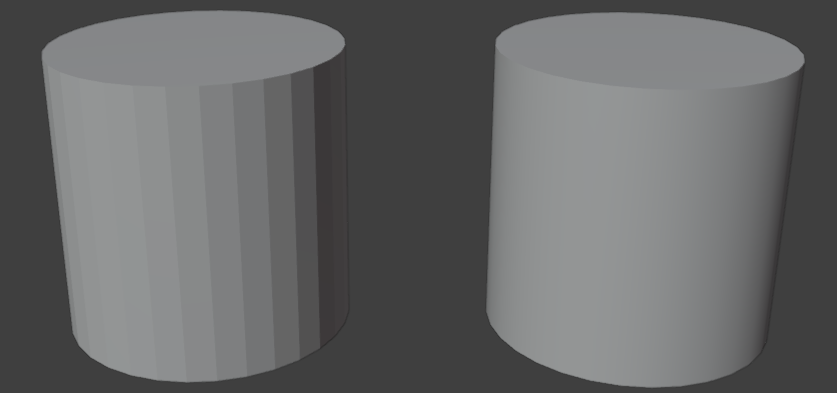
\includegraphics[width=0.7\columnwidth]{img/flat_smooth}
	\caption[Flat-Shading und Smooth-Shading]{Zwei Zylinder mit derselben Topologie und unterschiedliche Shading Arten in Blender. Links Flat-Shading und rechts Smooth-Shading mit der \dq Shade Auto Smooth\dq{} Funktion.}
	\label{fig:flat_smooth}
\end{figure}
\\
Nun gibt es zwei Ansätze für unterschiedliche Objektformen. Bei rechteckigen Objekten lohnt es sich den sogenannten \dq Bevel Modifier\dq{} zu verwenden. In der Abb. \ref{fig:bevel_cube} wird dieser als Beispiel auf einen Würfel angewendet. Dieser fügt an den äußeren Kanten neue Topologie hinzu, um diese abzurunden. Dadurch reflektiert das einfallende Licht deutlich natürlicher und das modellierte Objekt wirkt realistischer. Dafür reicht es schon wenige Kanten hinzuzufügen, wodurch die Menge an Vertices nur geringfügig steigt. 
\begin{figure} [ht]
	\centering
	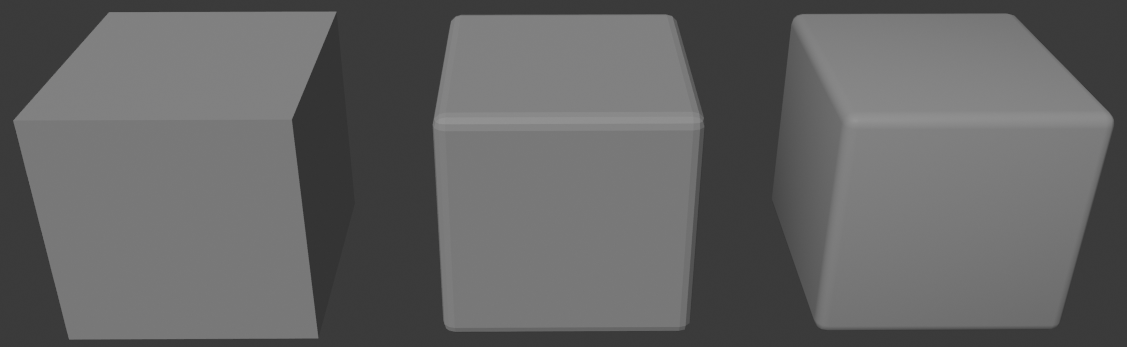
\includegraphics[width=\linewidth,height=\textheight,keepaspectratio]{img/bevel_cube}
	\caption[Visualisierung des Bevelmodifiers]{In der Abbildung sind drei Würfel dargestellt. Auf den zweiten und dritten ist der \dq Bevel Modifier\dq{} angewandt. Für den dritten Würfel wird dann noch Smooth-Shading verwendet.}
	\label{fig:bevel_cube}
\end{figure}
\\
Runde Modelle sind wiederum ein wenig komplizierter. Diese wirken bei genauerer Betrachtung erst rund, wenn die Anzahl an Kanten verhältnismäßig hoch ist. Dies führt automatisch dazu, dass runde Modelle mehr Vertices benötigen als Rechteckige. Hier muss eher beachtet werden aus welcher Entfernung das Objekt betrachtet wird und wie hoch die Auflösung sein sollte, damit die Kanten nicht auffallen. 
\\
Meine Erfahrung in diesem Bereich liefert mir ungefähre Anhaltspunkte, welche Anzahl an Vertices in Abhängigkeit von der Objektform gerechtfertigt sind. Für kleine rechteckige Objekte wie zum Beispiel die Artikel des Supermarktes habe ich mir eine Grenze von 1000 Vertices gesetzt. Runde Artikel hingegen können bis zu 3000 Vertices haben. Die Anzahl ist nicht besonders hoch und befindet sich eher im Low Poly Bereich.


\subsubsection{Visualisierung des Einkaufroboters}
\label{vis_agent}
Die vorher genannten Grenzen gelten jedoch nicht für Objekte, die eher im Fokus liegen wie der Roboter. Hier sind deutlich höher aufgelöste Topologien gerechtfertigt, da diese nur einmal pro Simulationsumgebung vorkommen. Für die Modellierung des Einkaufsroboters habe ich mir einen Prototypen des I-RobEka Projekts der TU Chemnitz als Anhaltspunkt ausgesucht siehe Abb. \ref{fig:robeka}.
\begin{figure} [ht]
	\centering
	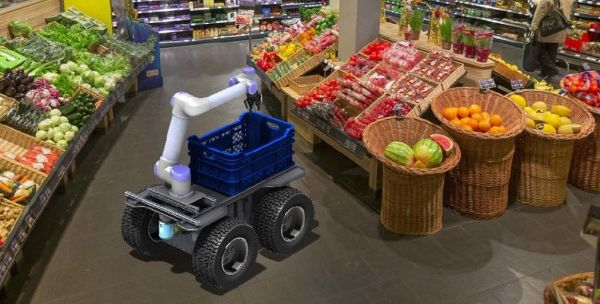
\includegraphics[width=0.8\columnwidth]{img/robeka}
	\caption[Ein Protoyp eines mobilen Roboters der TU Chemnitz]{Ein Prototyp des I-RobEka Projekts der TU Chemnitz\cite{robeka}.}
	\label{fig:robeka}
\end{figure}
\\
Der Roboter ist mit einem Greifarm ausgestattet und besitzt einen Korb, in dem die eingesammelten Objekte gelagert werden können. Des Weiteren ist ein Lidar im vorderen Bereich angebracht. Diese Elemente wurden für das eigene Modell übernommen, welches in der Abb. \ref{fig:robo} zu sehen ist. 
\begin{figure} [ht]
	\centering
	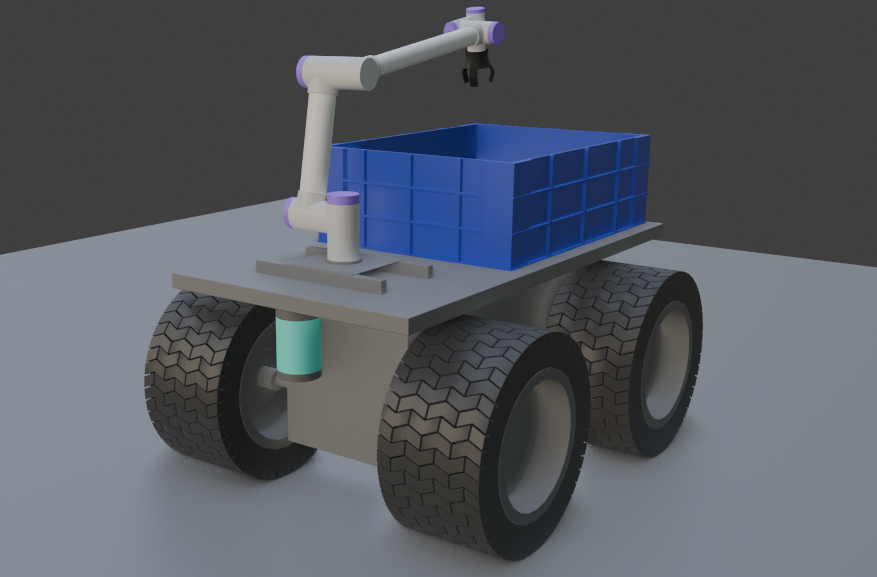
\includegraphics[width=0.75\columnwidth]{img/robo}
	\caption[Eigenes Roboter Modell]{Selbst modelliertes Roboter Modell mit dem TU Chemnitz Prototyp als Referenz.}
	\label{fig:robo}
\end{figure}
\\
Für den Roboter wurden gerundet 37000 Vertices verwendet und ca. 80000 Dreiecke. Um hier Einsparungen vorzunehmen, hätte man für das Reifenprofil eine Textur verwenden können. Das Profil wurde hier nämlich nachmodelliert. So wäre eine Halbierung der benutzten Vertices möglich. Jedoch liegt die Menge an Topologie für das Hauptmodell im Rahmen. 
\subsection{Generierung der dynamischen Umgebung}
Aus den Erkenntnissen von Kapitel \ref{annahmen} wird folgendes für die Simulation abgeleitet:
\\
\begin{itemize}
	\item der Abstand zwischen Regalen beträgt mindestens 2 Meter
	\item keine Sackgassen
	\item möglichst hohe Abdeckung mit Regalen
	\item quadratische oder rechteckige Umgebung mit vier verschiedenen Abteilen
	\item eine abgeschlossene Umgebung
\end{itemize}
\noindent
\\

